\begin{figure*}[t]
    \center
    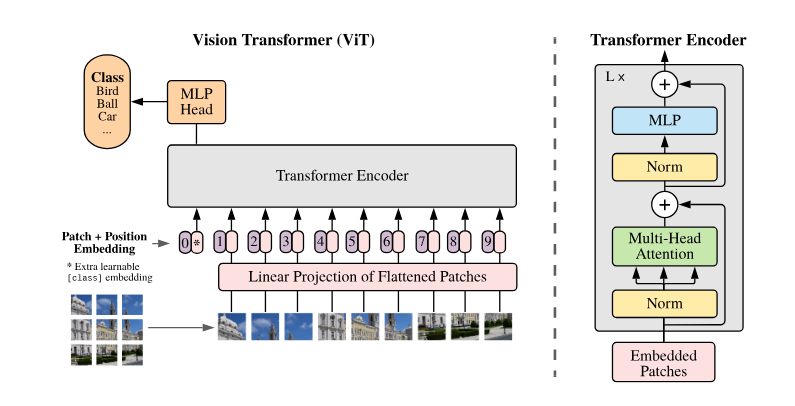
\includegraphics[width=1\textwidth]{images/vit-architecture.png}
    \caption{The Vision Transformer (ViT) architecture from \cite{alexey2020image}. On the left the model architecture while on the right the Transformer encoder block architecture from \cite{vaswani2017attention}.}
    \label{fig:vit-architecture}
\end{figure*}

\section{Architecture}

In recent years, the Transformer architecture—originally developed for natural language processing—has been successfully applied to computer vision tasks. The Vision Transformer (ViT) rethinks image classification by treating an image as a sequence of patches, much like tokens in a sentence, and processes them using standard Transformer blocks. In this chapter, we detail the architecture of the Vision Transformer and provide the mathematical foundations underlying its design.

\subsection{Overview}
The Vision Transformer (ViT) adapts the Transformer architecture—originally developed for natural language processing—to image classification tasks. Instead of processing an image as a whole, ViT divides it into a sequence of patches (analogous to tokens) and processes these patches through a stack of Transformer encoder blocks. The key steps in the ViT pipeline are:
\begin{enumerate}
    \item \textbf{Image Patch Embedding}: The input image is divided into fixed-size patches that are flattened and projected into a latent space.
    \item \textbf{Positional Encoding}: Since Transformers are permutation-invariant, positional embeddings are added to the patch embeddings.
    \item \textbf{Transformer Encoder}: A series of Transformer encoder blocks processes the sequence of embeddings using self-attention and feed-forward networks.
    \item \textbf{Classification Head}: The encoder output is used by a classification head for the final prediction.
\end{enumerate}

\subsection{Image Patch Embedding}

\textbf{Patch Extraction}

Given an input image 
\begin{equation}
    \mathbf{X} \in \mathbb{R}^{H \times W \times C},
\end{equation}
where \(H\) and \(W\) denote the height and width of the image, and \(C\) denotes the number of channels, the image is divided into \(N\) patches of size \(P \times P\). Hence, the number of patches is:
\begin{equation}
N = \frac{HW}{P^2}.
\end{equation}

\textbf{Flattening and Linear Projection}

Each patch, denoted as \(\mathbf{x}_p \in \mathbb{R}^{P \times P \times C}\), is flattened into a vector of dimension \(P^2 \cdot C\). A learnable linear projection (implemented as a fully connected layer) maps this vector into a \(D\)-dimensional embedding space:

\vspace{-\baselineskip} % Adjust spacing if needed
\begin{align}
    \mathbf{z}_p &= \mathbf{W}_e \mathbf{x}_p + \mathbf{b}_e, \nonumber \\
    \text{where } & \mathbf{W}_e \in \mathbb{R}^{D \times (P^2 \cdot C)} \text{ and } \mathbf{b}_e \in \mathbb{R}^{D}.
\end{align}
\vspace{-\baselineskip} % Adjust spacing if needed

After processing all patches, we obtain a sequence of embeddings:

\begin{equation}
\mathbf{Z} = \left[\mathbf{z}_1, \mathbf{z}_2, \dots, \mathbf{z}_N\right] \in \mathbb{R}^{N \times D}.
\end{equation}


